\chapter{Aplicação a dados de laboratório: amostra da cratera de Vredefort}
\label{sec:lab_application}

 

%% Figuras para aplicação a dados reais 
%\begin{figure}
%	\centering
%	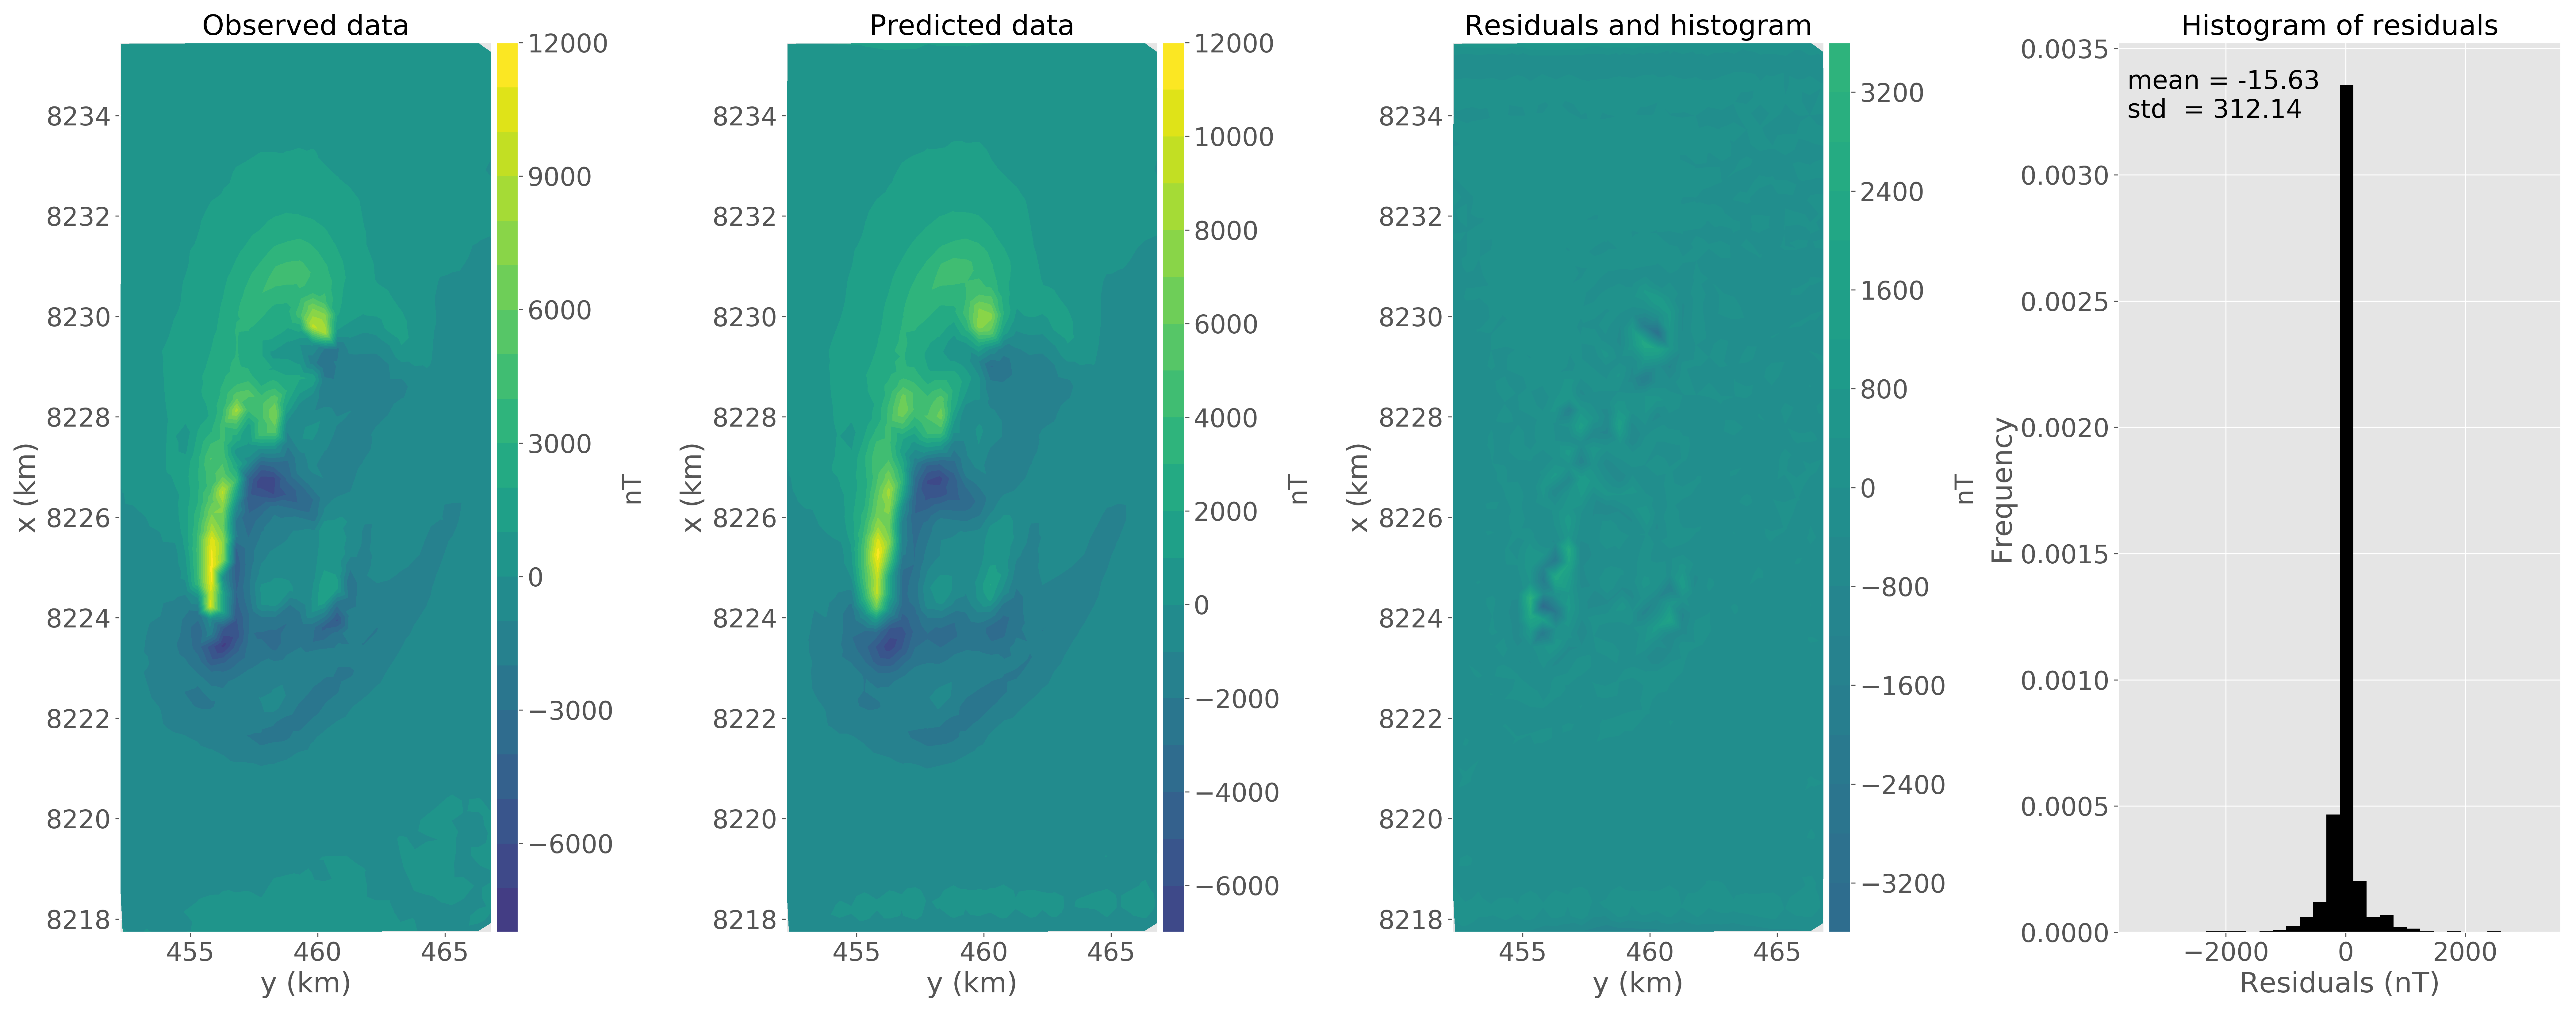
\includegraphics[width=1.1\textwidth]{Fig/eqlayer/field_data_montes_claros/data_fitting_LM_NNLS_montesclaros.png}
%	\caption{Aplicação a dados reais para o complexo de Montes Claros de Goiás. (a) Anomalia de campo total observada. (b) Dados preditos produzido pela camada equivalente. (c) Diferença entre os dados mostrados nos gráficos a e b. (d) Histograma dos resíduos.}
%	\label{fig:data_fitting_real}
%\end{figure}
%
%\begin{figure}
%	\centering
%	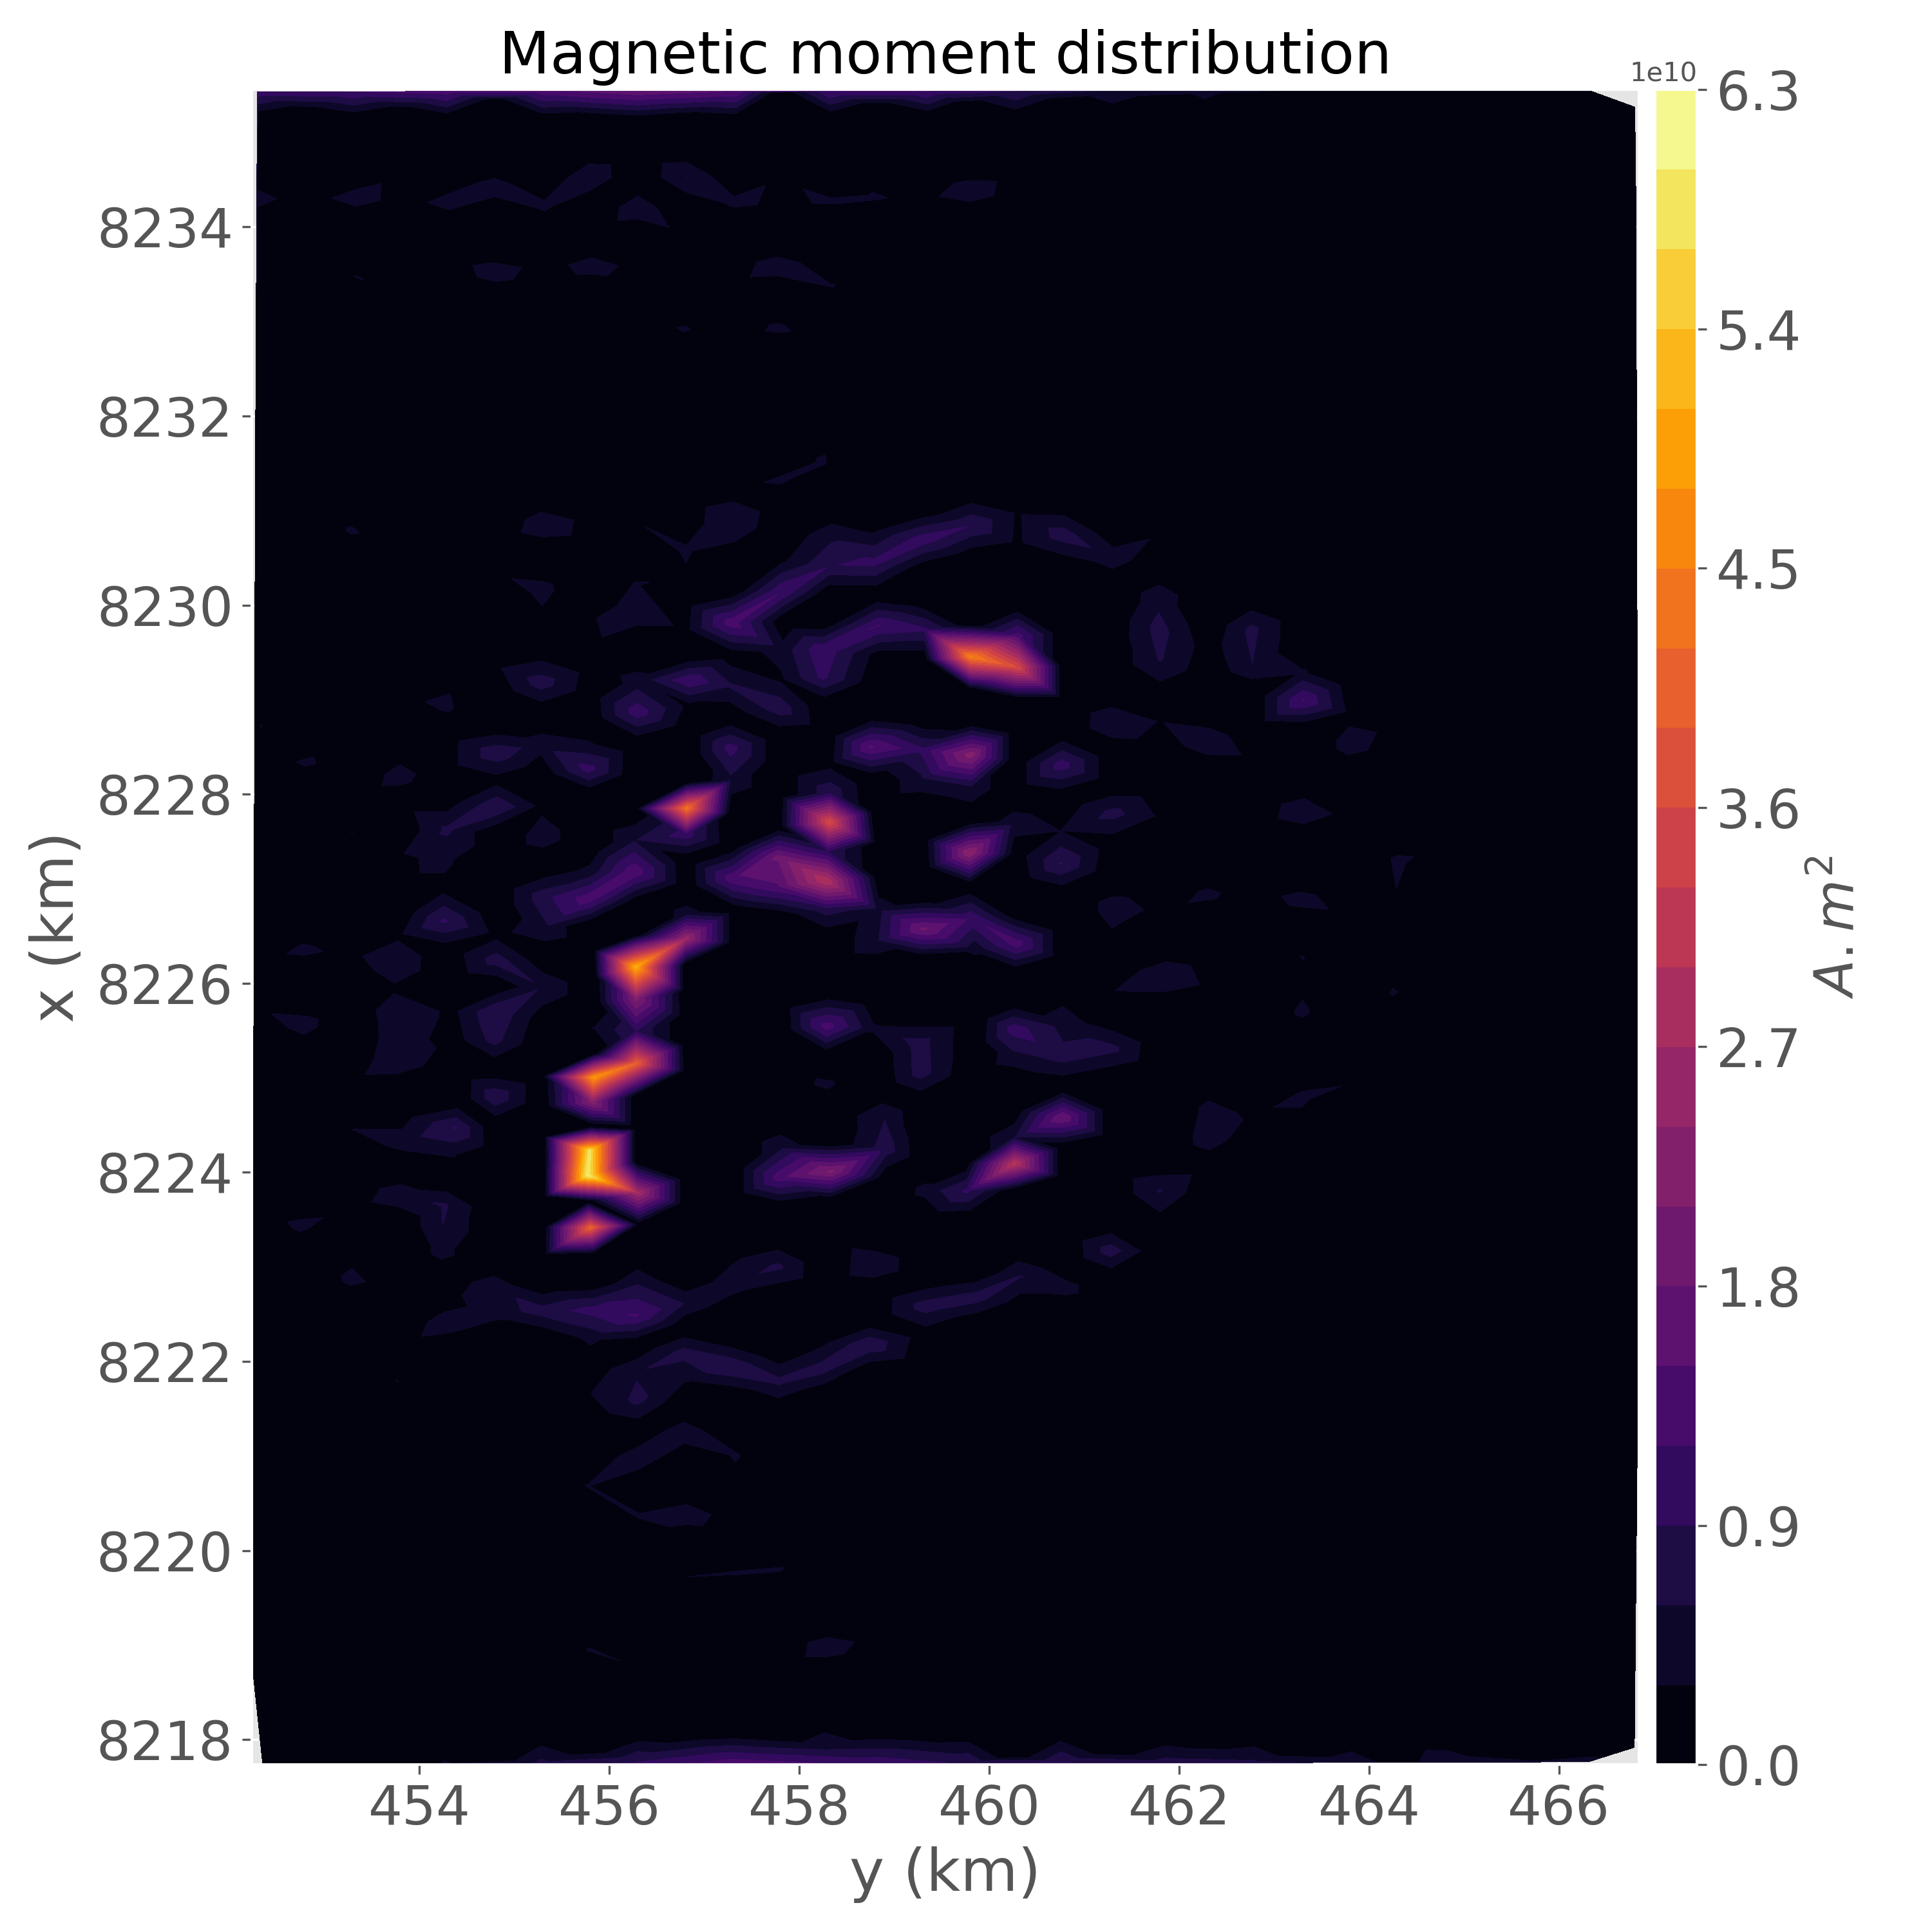
\includegraphics[width=.9\textwidth]{Fig/eqlayer/field_data_montes_claros/magnetic_moment_positive_LM_NNLS_montesclaros.png}
%	\caption{Distribuição de momentos magnéticos positiva para a aplicação a dados reais no complexo de Montes Claros de Goiás.}
%	\label{fig:dist_momentos_pos_real}
%\end{figure}
%
%\begin{figure}
%	\centering
%	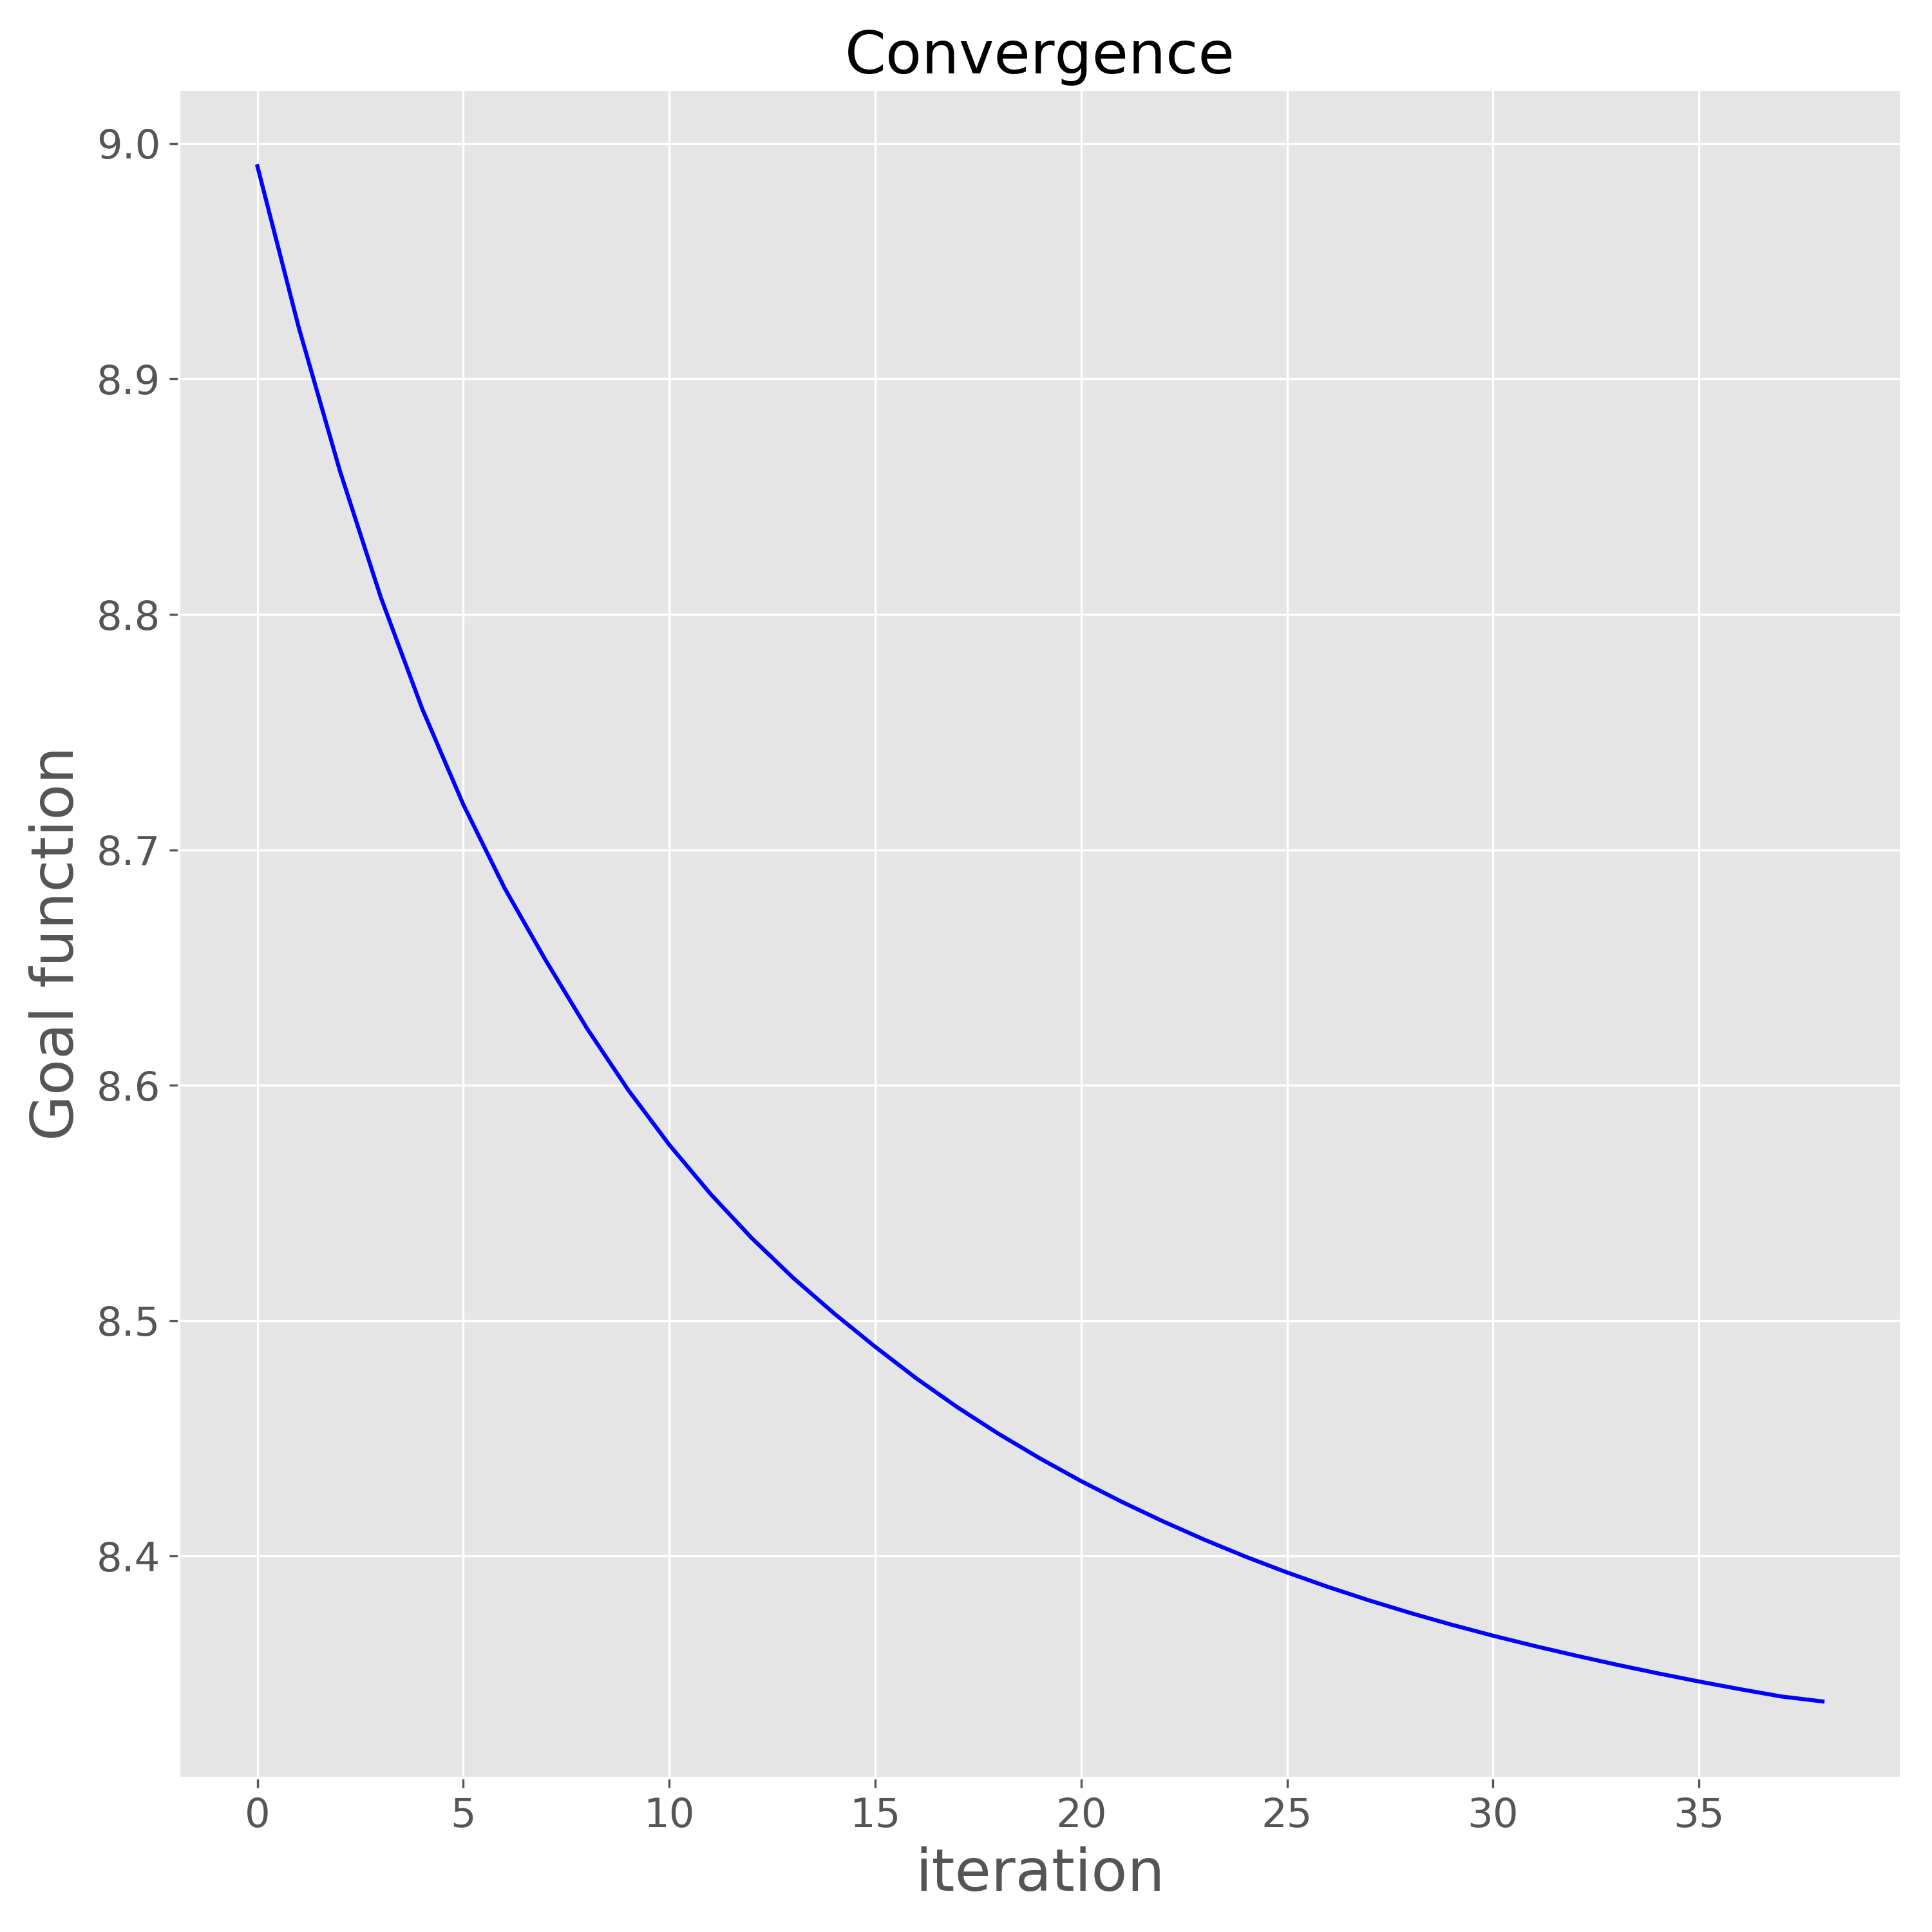
\includegraphics[width=.9\textwidth]{Fig/eqlayer/field_data_montes_claros/convergence_LM_NNLS_montesclaros.png}
%	\caption{Valor da função objetivo ao longo das iterações (equação \ref{eq:positivity_goal_function}a) mostrando a convergência do algoritmo.}
%	\label{fig:convergence_real}
%\end{figure}
%
%\begin{figure}
%	\centering
%	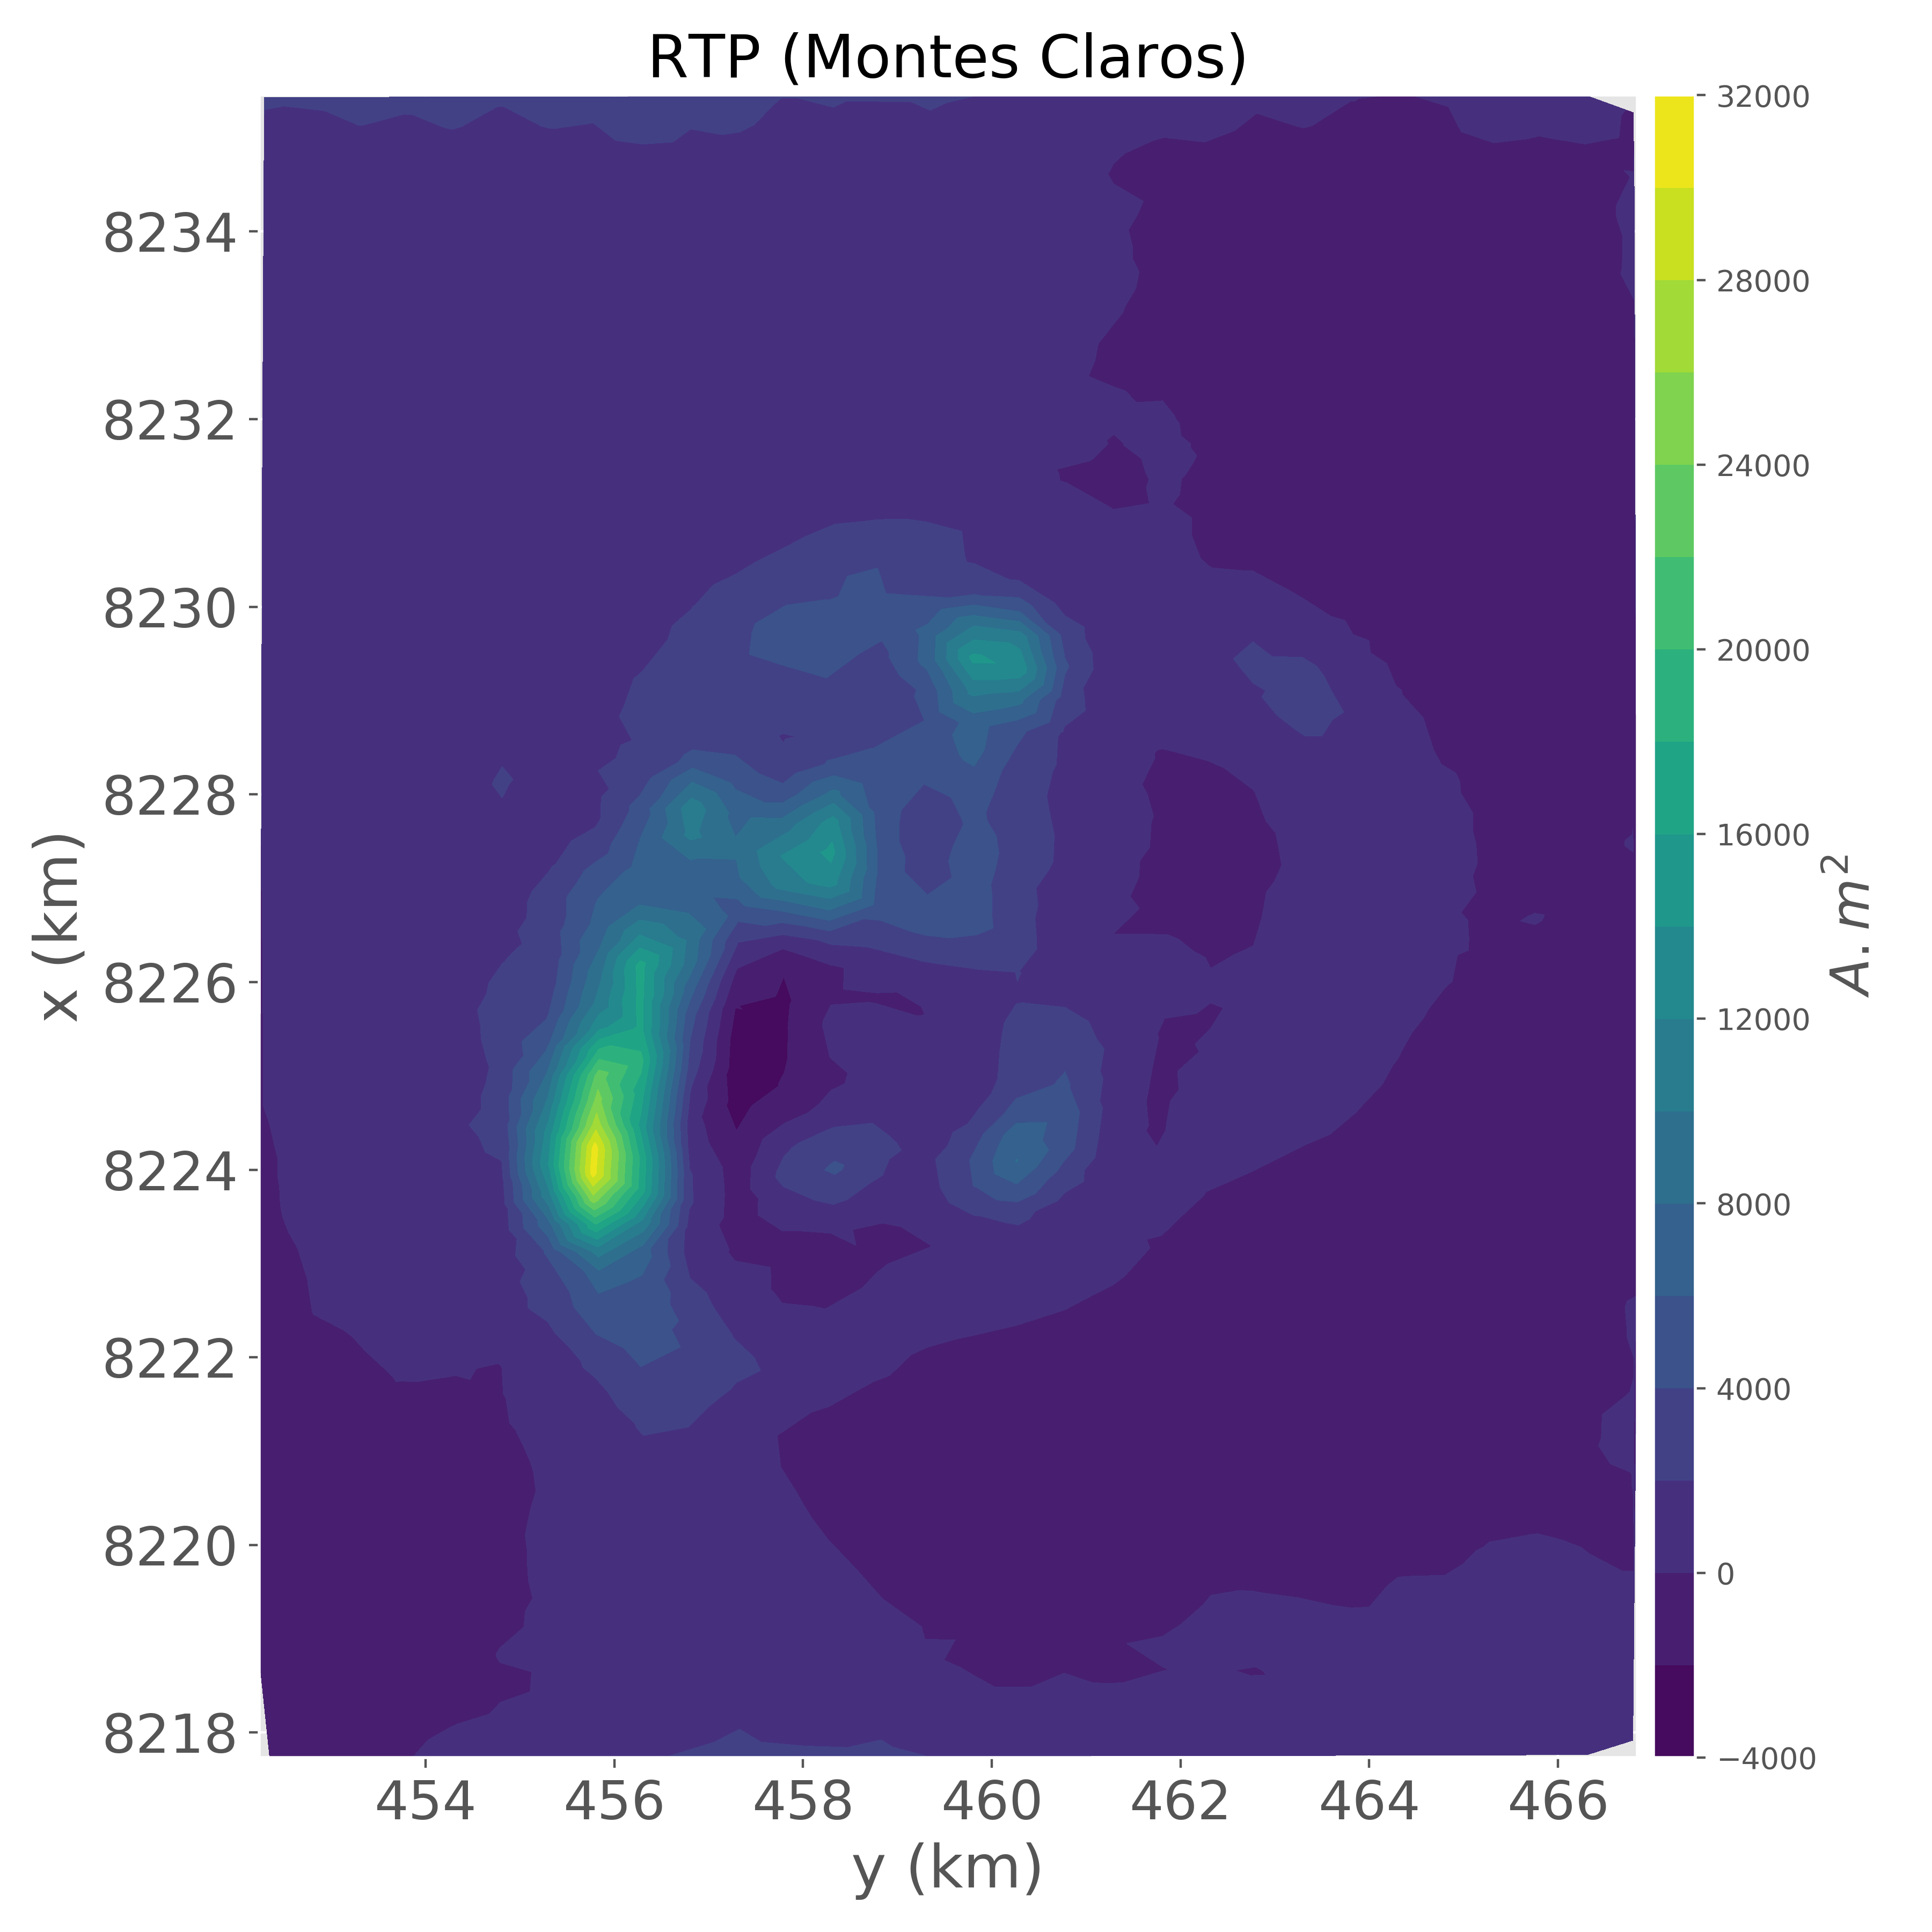
\includegraphics[width=.9\textwidth]{Fig/eqlayer/field_data_montes_claros/RTP_data_montes_claros.png}
%	\caption{Aplicação a dados reais no complexo de Montes Claros de Goiás utilizando a distribuição de momentos magnéticos estimada mostrada na figura \ref{fig:dist_momentos_pos_real}}
%	\label{fig:rtp_mc_data}
%\end{figure}

